\subsubsection{Estensione A: Campi Non Compilati o Compilati Erroneamente}

Durante la procedura di registrazione di un nuovo agente, il manager potrebbe tentare di completare l’operazione senza aver inserito tutti i dati richiesti o compilando alcuni campi in modo errato.
Per prevenire errori di input e garantire la coerenza delle informazioni salvate nel sistema, è previsto un controllo di validazione lato client.

\subsubsection{Gestione del Messaggio di Errore}
Nel momento in cui il manager clicca su \textbf{“Registra dipendente”} con uno o più campi incompleti o non validi, il sistema intercetta l’errore e mostra un messaggio specifico sotto ciascun campo non conforme.
Il messaggio indica chiaramente la tipologia di errore (es. campo obbligatorio, formato non valido, valore numerico errato), fornendo un feedback immediato e mirato.

L’interfaccia rimane attiva e consente al manager di correggere i dati direttamente nella stessa schermata, evitando la perdita delle informazioni già inserite.
Una volta completate le correzioni, il manager può ripetere l’operazione di registrazione, tornando così al flusso principale dello scenario (Step 3).

Questa soluzione progettuale segue i principi della \textbf{visibilità dello stato del sistema} e della \textbf{prevenzione degli errori} \cite{nielsen1995}, migliorando la comprensibilità e riducendo la frustrazione dell’utente.

\begin{figure}[H]
	\centering
	\begin{tikzpicture}[node distance=1.5cm and 1cm, auto]
		% Nodo per immagine 1 con didascalia sotto
		\node (img1) {
			\begin{tabular}{c}
				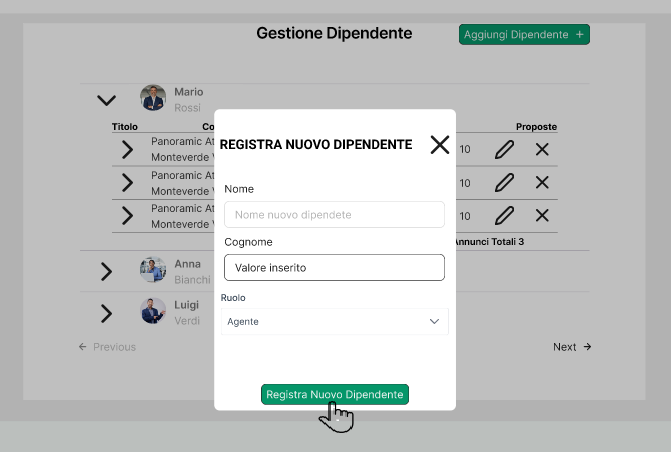
\includegraphics[width=0.7\textwidth]{Immagini/Mockup/nuovoAgente/extension A/nomeNonInserito.png} \\
				Cockburn: step 4.A
			\end{tabular}
		};
		
		% Nodo per immagine 2 con didascalia sotto, posizionato a destra di img1
		\node (img2) [below=of img1] {
			\begin{tabular}{c}
				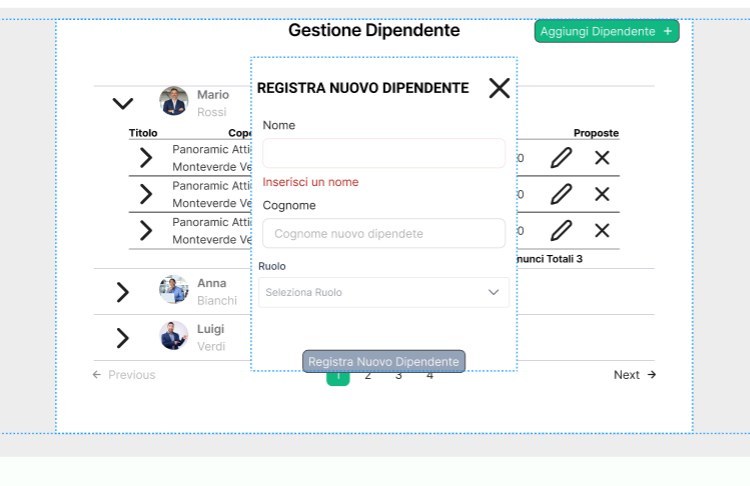
\includegraphics[width=0.7\textwidth]{Immagini/Mockup/nuovoAgente/extension A/messaggioDiErrore.png} \\
				Cockburn: step 5.A
			\end{tabular}
		};
	
		
		% Disegna le frecce
		\draw[->, thick] (img1) -- (img2);
		
	\end{tikzpicture}
	\caption{Mockup: Extension A della tabella di Cockburn del caso d'uso: Registra nuovo agente.}
	\label{fig:tikz_flow}
\end{figure}


